\newpage

\appendix \addcontentsline{toc}{section}{Appendix}

    \section{Appendix A: Schematics} \label{appendix:schematics}

        \begin{figure}[ht]
            \begin{center}
                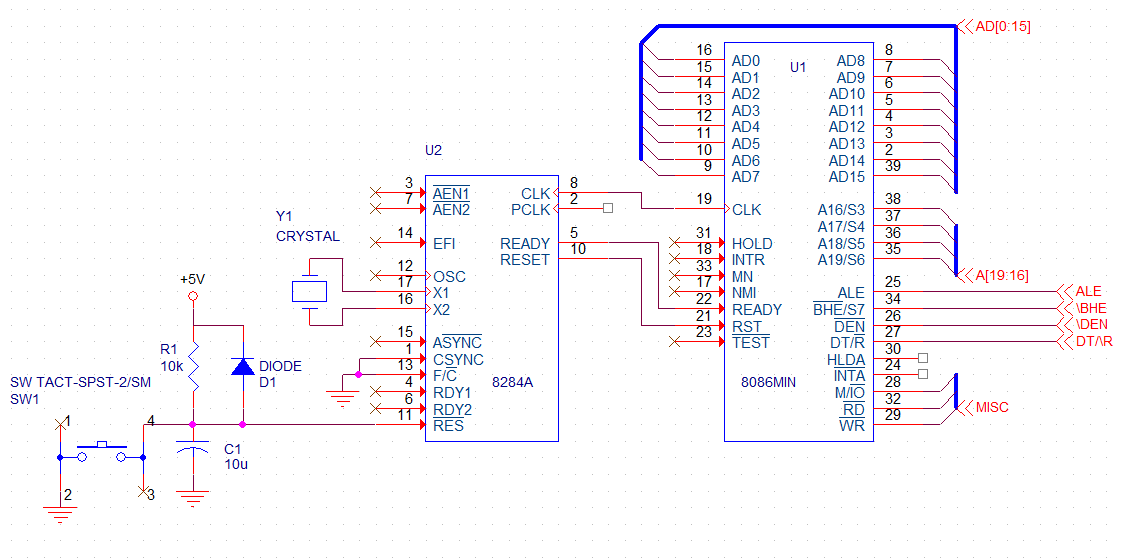
\includegraphics[width=0.95\textwidth]{figures/schematics/page1.png}
                \caption{8284A Interfaced with 8086 and its Reset RC Push Button Circuit} \label{fig:page1}
            \end{center}
        \end{figure}

        \begin{figure}[ht]
            \begin{center}
                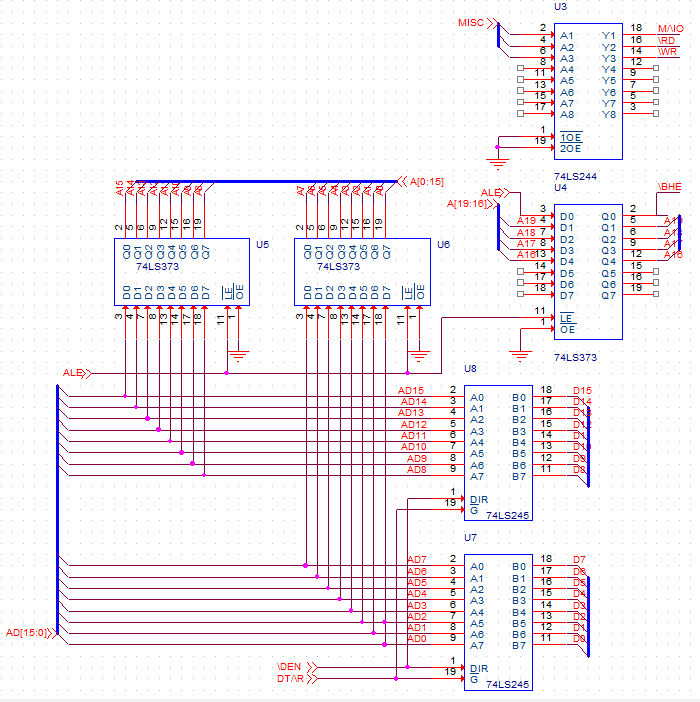
\includegraphics[width=0.95\textwidth]{figures/schematics/page2.png}
                \caption{8086 Demultiplexed} \label{fig:page2}
            \end{center}
        \end{figure}

        \begin{figure}[ht]
            \begin{center}
                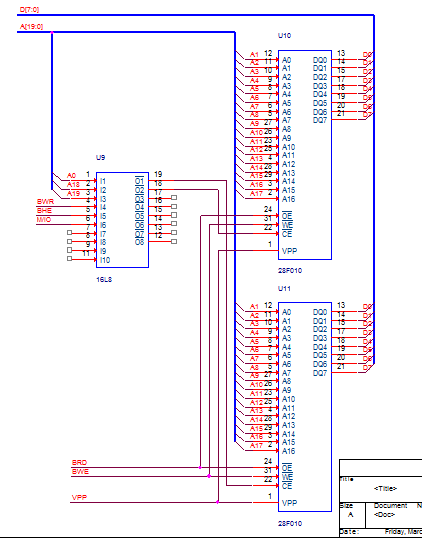
\includegraphics[width=0.95\textwidth]{figures/schematics/page3.png}
                \caption{8284A Interfaced with 8086 and its Reset RC Push Button Circuit} \label{fig:page3}
            \end{center}
        \end{figure}

        \begin{figure}[ht]
            \begin{center}
                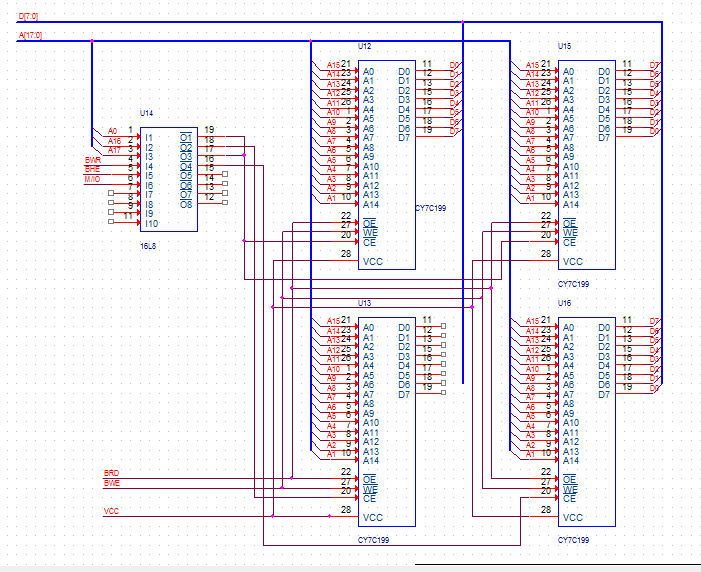
\includegraphics[width=0.95\textwidth]{figures/schematics/page4.png}
                \caption{8284A Interfaced with 8086 and its Reset RC Push Button Circuit} \label{fig:page4}
            \end{center}
        \end{figure}

        \begin{figure}[ht]
            \begin{center}
                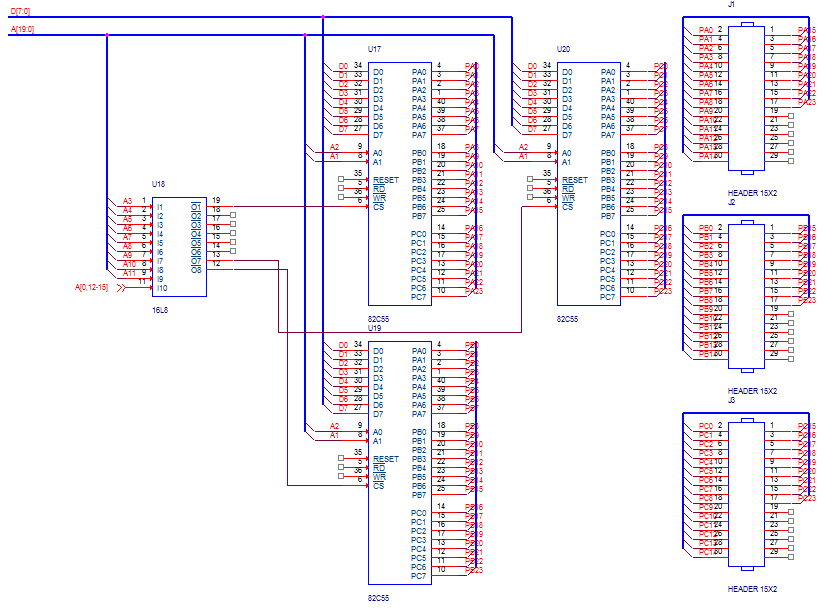
\includegraphics[width=0.95\textwidth]{figures/schematics/page5.png}
                \caption{8284A Interfaced with 8086 and its Reset RC Push Button Circuit} \label{fig:page5}
            \end{center}
        \end{figure}

        \begin{figure}[ht]
            \begin{center}
                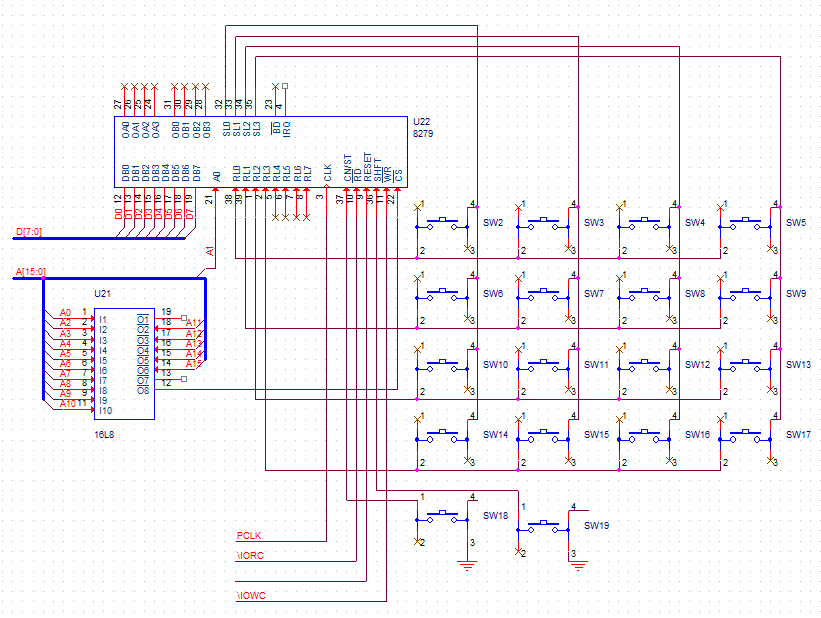
\includegraphics[width=0.95\textwidth]{figures/schematics/page6.png}
                \caption{8284A Interfaced with 8086 and its Reset RC Push Button Circuit} \label{fig:page6}
            \end{center}
        \end{figure}

        \begin{figure}[ht]
            \begin{center}
                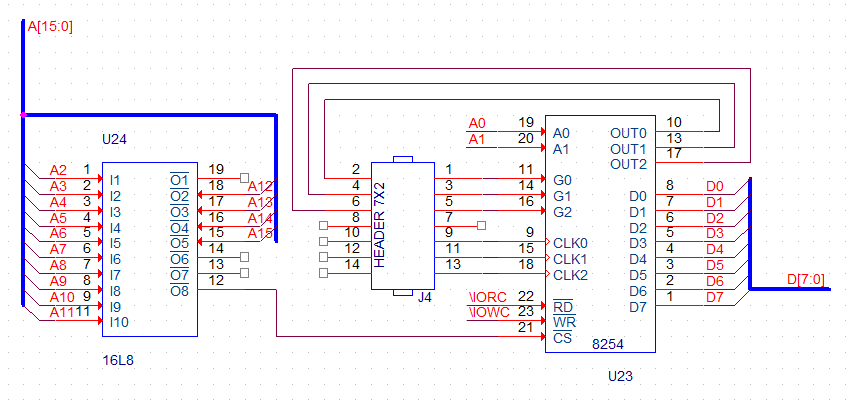
\includegraphics[width=0.95\textwidth]{figures/schematics/page7.png}
                \caption{8284A Interfaced with 8086 and its Reset RC Push Button Circuit} \label{fig:page7}
            \end{center}
        \end{figure}

        \begin{figure}[ht]
            \begin{center}
                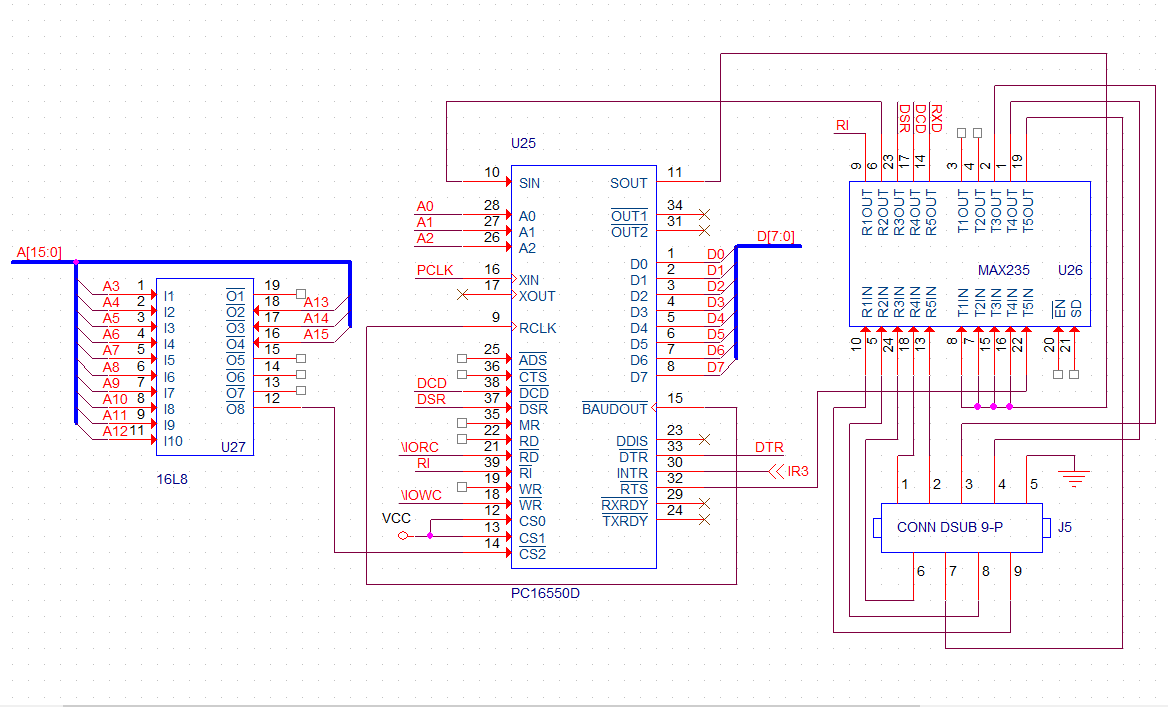
\includegraphics[width=0.95\textwidth]{figures/schematics/page8.png}
                \caption{8284A Interfaced with 8086 and its Reset RC Push Button Circuit} \label{fig:page8}
            \end{center}
        \end{figure}

        \begin{figure}[ht]
            \begin{center}
                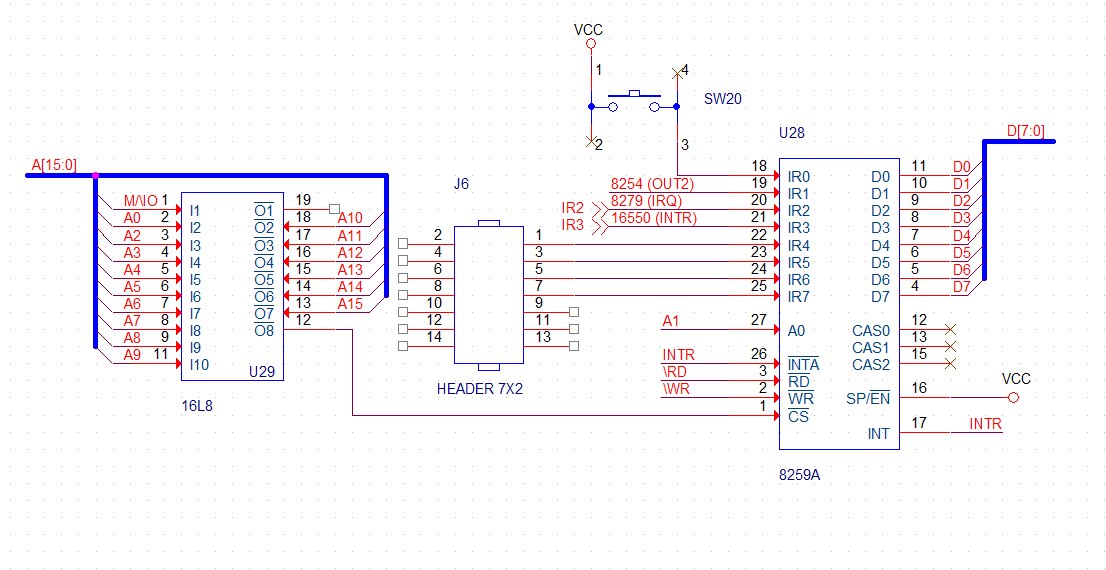
\includegraphics[width=0.95\textwidth]{figures/schematics/page9.png}
                \caption{8284A Interfaced with 8086 and its Reset RC Push Button Circuit} \label{fig:page9}
            \end{center}
        \end{figure}

        % \begin{figure}[ht]
        %     \begin{center}
        %         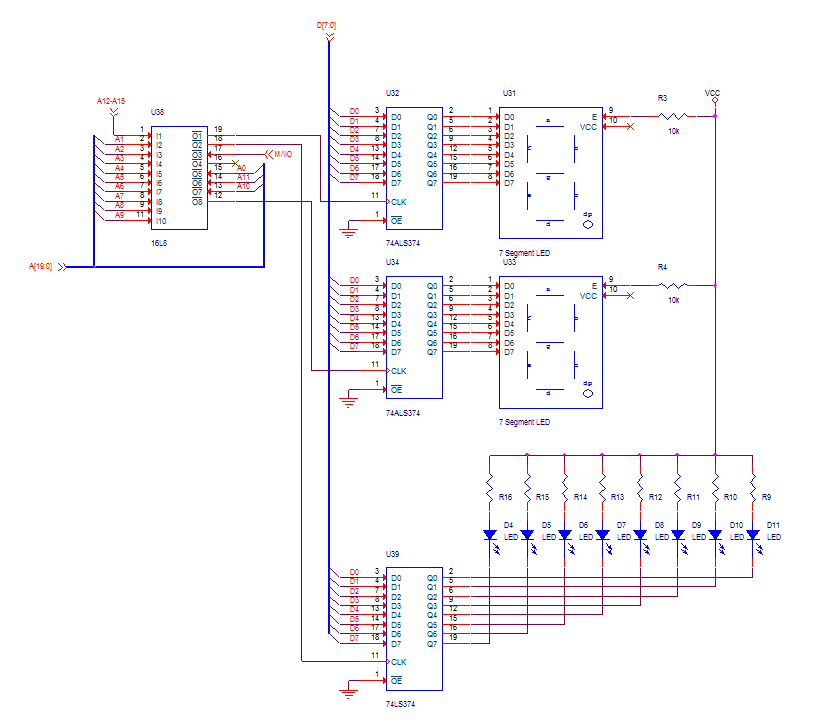
\includegraphics[width=0.95\textwidth]{figures/schematics/page10.png}
        %         \caption{8284A Interfaced with 8086 and its Reset RC Push Button Circuit} \label{fig:page10}
        %     \end{center}
        % \end{figure}



    \clearpage
    \newpage

    \section{Appendix B: Pinouts} \label{appendix:pinouts}

        \subsection{8086 Chip}

                \begin{itemize}

                    \item $M/\overline{IO}$: (Memory/ I/O) indicates if the address is a memory or I/O address

                    \item $\overline{INTA}$: (Interrupt Acknowledgment) generated in response to $INTR$ to put the interrupt vector on the data bus

                    \item $ALE$: (Address Latch Enable) when 1, address data bus contains a memory or I/O address

                    \item $\overline{DEN}$: (Data Bus Enable) activates external data bus buffers

                \end{itemize}
